%%%%%%%%%%%%%%%%%%%%%%%%%%%%%%%%%%%%%%%%%%%%%%%%%%%%%%%%%%%%%
%% APPENDICES
%%%%%%%%%%%%%%%%%%%%%%%%%%%%%%%%%%%%%%%%%%%%%%%%%%%%%%%%%%%%%
\appendix

\chapter{Appendix}
\label{app:acronyms}
%% acronyms
\printindex
\printglossaries

%\section{Data sets/Statistical Overview}
%\label{app:data_sets}

\clearpage
\section{MySQL Database}
\label{app:mysql_database}
% image of the mysql database
\begin{figure}[ht]
	\centering
    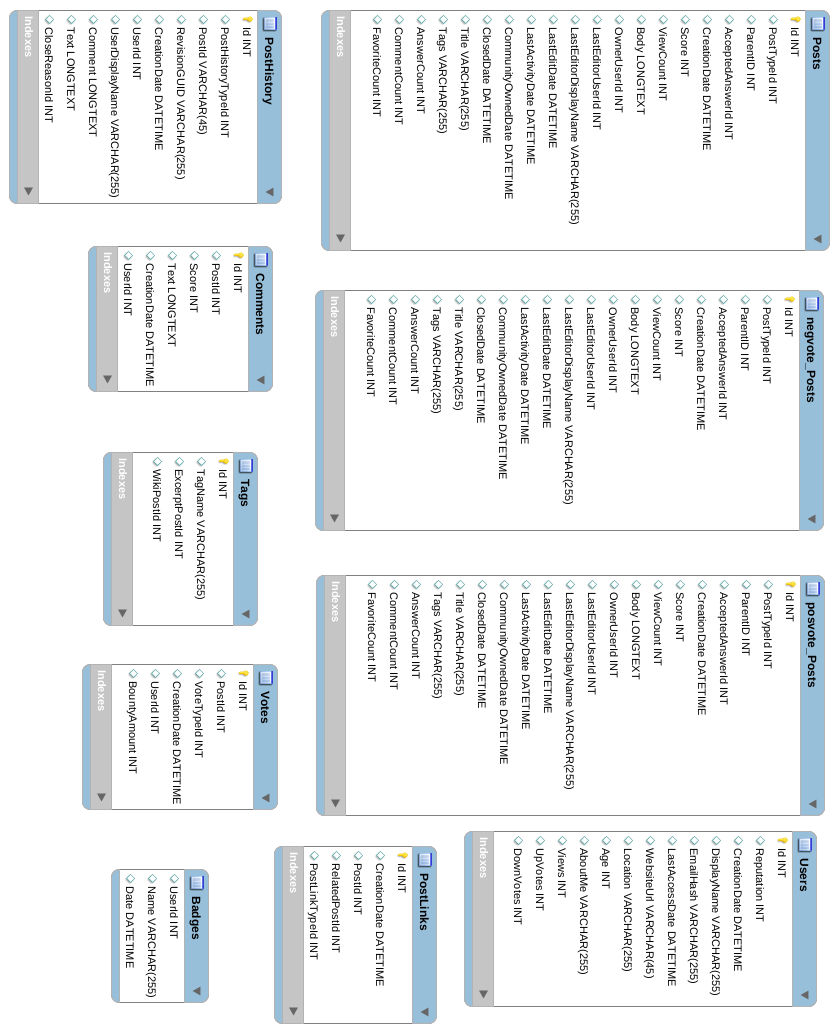
\includegraphics[width=0.8\textwidth]{so_database}
	\caption{MySQL Database used for dataset}
	\label{fig:mysql_database}
\end{figure}

\clearpage
\section{Confusion Matrices for Stack Overflow}
\label{app:confusion_matrix}
\subsection{Confusion matrices for unprocessed and all feature detectors}

\begin{table}[!htb]
	\caption{Confusion Matrix for unprocessed data set and all feature detectors using the same parameters.}
	\begin{minipage}{.5\linewidth}
		\caption{Unprocessed dataset}
		\centering
		\begin{tabular}{| c | c | c |}
			\hline
			Actual 		& Predicted: -1	& Predicted: 1	\\ \hline
			-1			& 1591			& 403			\\ \hline
			1			& 401			& 1605			\\ \hline
		\end{tabular}
	\end{minipage}%
	\begin{minipage}{.5\linewidth}
		\centering
		\caption{All features}
		\begin{tabular}{| c | c | c |}
			\hline
			Actual 		& Predicted: -1	& Predicted: 1	\\ \hline
			-1			& 1558			& 436			\\ \hline
			1			& 401			& 1605			\\ \hline
		\end{tabular}
	\end{minipage} 
	\begin{minipage}{.5\linewidth}
		\caption{Code blocks}
		\centering
		\begin{tabular}{| c | c | c |}
			\hline
			Actual 		& Predicted: -1	& Predicted: 1	\\ \hline
			-1			& 1547			& 420			\\ \hline
			1			& 413			& 1593			\\ \hline
		\end{tabular}
	\end{minipage}%
	\begin{minipage}{.5\linewidth}
		\centering
		\caption{Hexadecimal}
		\begin{tabular}{| c | c | c |}
			\hline
			Actual 		& Predicted: -1	& Predicted: 1	\\ \hline
			-1			& 1591			& 403			\\ \hline
			1			& 401			& 1605			\\ \hline
		\end{tabular}
	\end{minipage} 
	\begin{minipage}{.5\linewidth}
		\caption{Homework}
		\centering
		\begin{tabular}{| c | c | c |}
			\hline
			Actual 		& Predicted: -1	& Predicted: 1	\\ \hline
			-1			& 1590			& 404			\\ \hline
			1			& 400			& 1606			\\ \hline
		\end{tabular}
	\end{minipage}%
	\begin{minipage}{.5\linewidth}
		\centering
		\caption{Links}
		\begin{tabular}{| c | c | c |}
			\hline
			Actual 		& Predicted: -1	& Predicted: 1	\\ \hline
			-1			& 1548			& 410			\\ \hline
			1			& 416			& 1590			\\ \hline
		\end{tabular}
	\end{minipage} 	
	\begin{minipage}{.5\linewidth}
		\centering
		\caption{Numerical}
		\begin{tabular}{| c | c | c |}
			\hline
			Actual 		& Predicted: -1	& Predicted: 1	\\ \hline
			-1			& 1591			& 403			\\ \hline
			1			& 375			& 1631			\\ \hline
		\end{tabular}
	\end{minipage}%	
	\begin{minipage}{.5\linewidth}
		\caption{Tags}
		\centering
		\begin{tabular}{| c | c | c |}
			\hline
			Actual 		& Predicted: -1	& Predicted: 1	\\ \hline
			-1			& 1508			& 486			\\ \hline
			1			& 467			& 1539			\\ \hline
		\end{tabular}
	\end{minipage}
\end{table}	


\begin{table}[!htb]
	\caption{Confusion Matrix for all features, with and without stemming.}
	\begin{minipage}{.5\linewidth}
		\caption{With stemming}
		\centering
		\begin{tabular}{| c | c | c |}
			\hline
			Actual 		& Predicted: -1	& Predicted: 1	\\ \hline
			-1			& 1558			& 436				\\ \hline
			1			& 525			& 1481				\\ \hline
		\end{tabular}
	\end{minipage}%
	\begin{minipage}{.5\linewidth}
		\centering
		\caption{Without stemming}
		\begin{tabular}{| c | c | c |}
			\hline
			Actual 		& Predicted: -1	& Predicted: 1	\\ \hline
			-1			& 1567			& 427				\\ \hline
			1			& 408			& 1598				\\ \hline
		\end{tabular}
	\end{minipage} 
\end{table}	
\begin{table}[!htb]
	\caption{Confusion Matrix for the SGD classifier, with loss='log'.}
	\begin{minipage}{.5\linewidth}
		\caption{Unprocessed}
		\centering
		\begin{tabular}{| c | c | c |}
			\hline
			Actual 		& Predicted: -1	& Predicted: 1	\\ \hline
			-1			& 1607			& 387			\\ \hline
			1			& 418			& 1588			\\ \hline
		\end{tabular}
	\end{minipage}%
	\begin{minipage}{.5\linewidth}
		\caption{All features with stemming}
		\centering
		\begin{tabular}{| c | c | c |}
			\hline
			Actual 		& Predicted: -1	& Predicted: 1	\\ \hline
			-1			& 1610			& 384			\\ \hline
			1			& 594			& 1412			\\ \hline
		\end{tabular}
	\end{minipage} 
\end{table}	




\begin{comment}
\clearpage
%\subsection{Confusion matrix for singular feature detectors - all questions}

\begin{table}[!htb]
	\caption{Confusion Matrix for singular feature detectors, based on all questions in the data set.}	
	\begin{minipage}{.5\linewidth}
		\caption{Code blocks}
		\centering
		\begin{tabular}{| c | c | c |}
			\hline
			Actual 		& Predicted: -1	& Predicted: 1	\\ \hline
			-1			& 1547			& 420			\\ \hline
			1			& 413			& 1593			\\ \hline
		\end{tabular}
	\end{minipage}%
	\begin{minipage}{.5\linewidth}
		\centering
		\caption{Hexadecimal}
		\begin{tabular}{| c | c | c |}
			\hline
			Actual 		& Predicted: -1	& Predicted: 1	\\ \hline
			-1			& 1591			& 403			\\ \hline
			1			& 401			& 1605			\\ \hline
		\end{tabular}
	\end{minipage} 
	\begin{minipage}{.5\linewidth}
		\caption{Homework}
		\centering
		\begin{tabular}{| c | c | c |}
			\hline
			Actual 		& Predicted: -1	& Predicted: 1	\\ \hline
			-1			& 1590			& 404			\\ \hline
			1			& 400			& 1606			\\ \hline
		\end{tabular}
	\end{minipage}%
	\begin{minipage}{.5\linewidth}
		\centering
		\caption{Links}
		\begin{tabular}{| c | c | c |}
			\hline
			Actual 		& Predicted: -1	& Predicted: 1	\\ \hline
			-1			& 1548			& 410			\\ \hline
			1			& 416			& 1590			\\ \hline
		\end{tabular}
	\end{minipage} 	
	\begin{minipage}{.5\linewidth}
		\centering
		\caption{Numerical}
		\begin{tabular}{| c | c | c |}
			\hline
			Actual 		& Predicted: -1	& Predicted: 1	\\ \hline
			-1			& 1591			& 403			\\ \hline
			1			& 375			& 1631			\\ \hline
		\end{tabular}
	\end{minipage}%	
	\begin{minipage}{.5\linewidth}
		\caption{Tags}
		\centering
		\begin{tabular}{| c | c | c |}
			\hline
			Actual 		& Predicted: -1	& Predicted: 1	\\ \hline
			-1			& 1508			& 486			\\ \hline
			1			& 467			& 1539			\\ \hline
		\end{tabular}
	\end{minipage}
\end{table}	

\end{comment}

\clearpage
\subsection{Confusion matrices for singular feature detectors - occurrence only}
\label{app:conf_matrix_singular_only}

\begin{table}[!htb]
	\caption{Confusion Matrix for singular feature detectors, only for questions containing it.}
	\begin{minipage}{.5\linewidth}
		\caption{Unprocessed}
		\centering
		\begin{tabular}{| c | c | c |}
			\hline
			Actual 		& Predicted: -1	& Predicted: 1	\\ \hline
			-1			& 786			& 202			\\ \hline
			1			& 215			& 768				\\ \hline
		\end{tabular}
	\end{minipage}%
	\begin{minipage}{.5\linewidth}
		\centering
		\caption{Code blocks}
		\begin{tabular}{| c | c | c |}
			\hline
			Actual 		& Predicted: -1	& Predicted: 1	\\ \hline
			-1			& 793			& 195			\\ \hline
			1			& 218			& 765				\\ \hline
		\end{tabular}
	\end{minipage}
	\begin{minipage}{.5\linewidth}
		\caption{Unprocessed}
		\centering
		\begin{tabular}{| c | c | c |}
			\hline
			Actual 		& Predicted: -1	& Predicted: 1	\\ \hline
			-1			& 21			& 0			\\ \hline
			1			& 6				& 5				\\ \hline
		\end{tabular}
	\end{minipage}%
	\begin{minipage}{.5\linewidth}
		\centering
		\caption{Hexadecimal}
		\begin{tabular}{| c | c | c |}
			\hline
			Actual 		& Predicted: -1	& Predicted: 1	\\ \hline
			-1			& 21			& 0				\\ \hline
			1			& 6				& 5				\\ \hline
		\end{tabular}
	\end{minipage} 	
	\begin{minipage}{.5\linewidth}
		\centering
		\caption{Unprocessed}
		\begin{tabular}{| c | c | c |}
			\hline
			Actual 		& Predicted: -1	& Predicted: 1	\\ \hline
			-1			& 52			& 4			\\ \hline
			1			& 8				& 11		\\ \hline
		\end{tabular}
	\end{minipage} 	%
	\begin{minipage}{.5\linewidth}
		\caption{Homework}
		\centering
		\begin{tabular}{| c | c | c |}
			\hline
			Actual 		& Predicted: -1	& Predicted: 1	\\ \hline
			-1			& 50			& 6 			\\ \hline
			1			& 7 			& 12			\\ \hline
		\end{tabular}
	\end{minipage}
	\begin{minipage}{.5\linewidth}
		\caption{Unprocessed}
		\centering
		\begin{tabular}{| c | c | c |}
			\hline
			Actual 		& Predicted: -1	& Predicted: 1	\\ \hline
			-1			& 95			& 56			\\ \hline
			1			& 28			& 337			\\ \hline
		\end{tabular}
	\end{minipage}%
	\begin{minipage}{.5\linewidth}
		\centering
		\caption{Links}
		\begin{tabular}{| c | c | c |}
			\hline
			Actual 		& Predicted: -1	& Predicted: 1	\\ \hline
			-1			& 87			& 64			\\ \hline
			1			& 30			& 335			\\ \hline
		\end{tabular}
	\end{minipage} 
	\begin{minipage}{.5\linewidth}
		\caption{Unprocessed}
		\centering
		\begin{tabular}{| c | c | c |}
			\hline
			Actual 		& Predicted: -1	& Predicted: 1	\\ \hline
			-1			& 1044			& 110			\\ \hline
			1			& 247			& 404			\\ \hline
		\end{tabular}
	\end{minipage}%
	\begin{minipage}{.5\linewidth}
		\centering
		\caption{Numerical}
		\begin{tabular}{| c | c | c |}
			\hline
			Actual 		& Predicted: -1	& Predicted: 1	\\ \hline
			-1			& 1043			& 111			\\ \hline
			1			& 256			& 395			\\ \hline
		\end{tabular}
	\end{minipage} 	
	\begin{minipage}{.5\linewidth}
		\centering
		\caption{Unprocessed}
		\begin{tabular}{| c | c | c |}
			\hline
			Actual 		& Predicted: -1	& Predicted: 1	\\ \hline
			-1			& 1559			& 426			\\ \hline
			1			& 398			& 1611			\\ \hline
		\end{tabular}
	\end{minipage}%
	\begin{minipage}{.5\linewidth}
		\caption{Tags}
		\centering
		\begin{tabular}{| c | c | c |}
			\hline
			Actual 		& Predicted: -1	& Predicted: 1	\\ \hline
			-1			& 1487			& 498			\\ \hline
			1			& 442			& 1567			\\ \hline
		\end{tabular}
	\end{minipage}
	\begin{minipage}{.5\linewidth}
		\caption{Unprocessed}
		\centering
		\begin{tabular}{| c | c | c |}
			\hline
			Actual 		& Predicted: -1	& Predicted: 1	\\ \hline
			-1			& 1284			& 387			\\ \hline
			1			& 342			& 1499			\\ \hline
		\end{tabular}
	\end{minipage}%
	\begin{minipage}{.5\linewidth}
		\caption{All features}
		\centering
		\begin{tabular}{| c | c | c |}
			\hline
			Actual 		& Predicted: -1	& Predicted: 1	\\ \hline
			-1			& 1268			& 403			\\ \hline
			1			& 329			& 1512			\\ \hline
		\end{tabular}
	\end{minipage}
\end{table}	

\begin{comment}
\section{Classification report for Stack Overflow}

\begin{table}[!htb]
	\caption{Classification report for unprocessed data set and all feature detectors using the same parameters.}
	\begin{minipage}{.5\linewidth}
		\caption{Unprocessed dataset}
		\centering
		\begin{tabular}{| c | c | c | c | c |}
			\hline
			~				& Precision		& Recall	& F1-score		& Support	\\ \hline
			-1      		& xxxx			& xxxx		& xxxx			& xxxx		\\ \hline
			1       		& xxxx			& xxxx		& 1x00			& xxxx		\\ \hline
			avg/total		& xxxx			& xxxx		& xxxx			& xxxx		\\ \hline
		\end{tabular}
	\end{minipage}%
	\begin{minipage}{.5\linewidth}
		\centering
		\caption{All features}
		\begin{tabular}{| c | c | c | c | c |}
			\hline
			Precision		& Recall	& F1-score		& Support	\\ \hline
			xxxx			& xxxx		& xxxx			& xxxx		\\ \hline
			xxxx			& xxxx		& 1x00			& xxxx		\\ \hline
			xxxx			& xxxx		& xxxx			& xxxx		\\ \hline
		\end{tabular}
	\end{minipage} 
	\begin{minipage}{.5\linewidth}
		\caption{Code blocks}
		\centering
		\begin{tabular}{| c | c | c | c | c |}
			\hline
			~				& Precision		& Recall	& F1-score		& Support	\\ \hline
			-1      		& xxxx			& xxxx		& xxxx			& xxxx		\\ \hline
			1       		& xxxx			& xxxx		& 1x00			& xxxx		\\ \hline
			avg / total		& xxxx			& xxxx		& xxxx			& xxxx		\\ \hline
		\end{tabular}
	\end{minipage}%
	\begin{minipage}{.5\linewidth}
		\centering
		\caption{Hexadecimal}
		\begin{tabular}{| c | c | c | c | c |}
			\hline
			~				& Precision		& Recall	& F1-score		& Support	\\ \hline
			-1      		& xxxx			& xxxx		& xxxx			& xxxx		\\ \hline
			1       		& xxxx			& xxxx		& 1x00			& xxxx		\\ \hline
			avg / total		& xxxx			& xxxx		& xxxx			& xxxx		\\ \hline
		\end{tabular}
	\end{minipage} 
	\begin{minipage}{.5\linewidth}
		\caption{Homework}
		\centering
		\begin{tabular}{| c | c | c | c | c |}
			\hline
			~				& Precision		& Recall	& F1-score		& Support	\\ \hline
			-1      		& xxxx			& xxxx		& xxxx			& xxxx		\\ \hline
			1       		& xxxx			& xxxx		& 1x00			& xxxx		\\ \hline
			avg / total		& xxxx			& xxxx		& xxxx			& xxxx		\\ \hline
		\end{tabular}
	\end{minipage}%
	\begin{minipage}{.5\linewidth}
		\centering
		\caption{Links}
		\begin{tabular}{| c | c | c | c | c |}
			\hline
			~				& Precision		& Recall	& F1-score		& Support	\\ \hline
			-1      		& xxxx			& xxxx		& xxxx			& xxxx		\\ \hline
			1       		& xxxx			& xxxx		& 1x00			& xxxx		\\ \hline
			avg / total		& xxxx			& xxxx		& xxxx			& xxxx		\\ \hline
		\end{tabular}
	\end{minipage} 	
	\begin{minipage}{.5\linewidth}
		\centering
		\caption{Numerical}
		\begin{tabular}{| c | c | c | c | c |}
			\hline
			~				& Precision		& Recall	& F1-score		& Support	\\ \hline
			-1      		& xxxx			& xxxx		& xxxx			& xxxx		\\ \hline
			1       		& xxxx			& xxxx		& 1x00			& xxxx		\\ \hline
			avg / total		& xxxx			& xxxx		& xxxx			& xxxx		\\ \hline
		\end{tabular}
	\end{minipage}%	
	\begin{minipage}{.5\linewidth}
		\caption{Tags}
		\centering
		\begin{tabular}{| c | c | c | c | c |}
			\hline
			~				& Precision		& Recall	& F1-score		& Support	\\ \hline
			-1      		& xxxx			& xxxx		& xxxx			& xxxx		\\ \hline
			1       		& xxxx			& xxxx		& 1x00			& xxxx		\\ \hline
			avg / total		& xxxx			& xxxx		& xxxx			& xxxx		\\ \hline
		\end{tabular}
	\end{minipage}
\end{table}	


\begin{table}[!htb]
	\caption{Classification report for all features, with and without stemming.}
	\begin{minipage}{.5\linewidth}
		\caption{With stemming}
		\centering
		\begin{tabular}{| c | c | c | c | c |}
			\hline
			~				& Precision		& Recall	& F1-score		& Support	\\ \hline
			-1      		& xxxx			& xxxx		& xxxx			& xxxx		\\ \hline
			1       		& xxxx			& xxxx		& 1x00			& xxxx		\\ \hline
			avg / total		& xxxx			& xxxx		& xxxx			& xxxx		\\ \hline
		\end{tabular}
	\end{minipage}%
	\begin{minipage}{.5\linewidth}
		\centering
		\caption{Without stemming}
		\begin{tabular}{| c | c | c | c | c |}
			\hline
			~				& Precision		& Recall	& F1-score		& Support	\\ \hline
			-1      		& xxxx			& xxxx		& xxxx			& xxxx		\\ \hline
			1       		& xxxx			& xxxx		& 1x00			& xxxx		\\ \hline
			avg / total		& xxxx			& xxxx		& xxxx			& xxxx		\\ \hline
		\end{tabular}
	\end{minipage} 
\end{table}	
\begin{table}[!htb]
	\caption{Confusion Matrix for the SGD classifier, with loss='log'.}
	\begin{minipage}{.5\linewidth}
		\caption{Unprocessed}
		\centering
		\begin{tabular}{| c | c | c | c | c |}
			\hline
			~				& Precision		& Recall	& F1-score		& Support	\\ \hline
			-1      		& xxxx			& xxxx		& xxxx			& xxxx		\\ \hline
			1       		& xxxx			& xxxx		& 1x00			& xxxx		\\ \hline
			avg / total		& xxxx			& xxxx		& xxxx			& xxxx		\\ \hline
		\end{tabular}
	\end{minipage}%
	\begin{minipage}{.5\linewidth}
		\caption{All features with stemming}
		\centering
		\begin{tabular}{| c | c | c | c | c |}
			\hline
			~				& Precision		& Recall	& F1-score		& Support	\\ \hline
			-1      		& xxxx			& xxxx		& xxxx			& xxxx		\\ \hline
			1       		& xxxx			& xxxx		& 1x00			& xxxx		\\ \hline
			avg / total		& xxxx			& xxxx		& xxxx			& xxxx		\\ \hline
		\end{tabular}
	\end{minipage} 
\end{table}	

\clearpage
\subsection{Classification report for singular feature detectors - occurrence only}

\begin{table}[!htb]
	\caption{Classification report for singular feature detectors, only for questions containing it.}
	\begin{minipage}{.5\linewidth}
		\caption{Unprocessed}
		\centering
		\begin{tabular}{| c | c | c | c | c |}
			\hline
			~				& Precision		& Recall	& F1-score		& Support	\\ \hline
			-1      		& xxxx			& xxxx		& xxxx			& xxxx		\\ \hline
			1       		& xxxx			& xxxx		& 1x00			& xxxx		\\ \hline
			avg / total		& xxxx			& xxxx		& xxxx			& xxxx		\\ \hline
		\end{tabular}
	\end{minipage}%
	\begin{minipage}{.5\linewidth}
		\centering
		\caption{Code blocks}
		\begin{tabular}{| c | c | c | c | c |}
			\hline
			~				& Precision		& Recall	& F1-score		& Support	\\ \hline
			-1      		& xxxx			& xxxx		& xxxx			& xxxx		\\ \hline
			1       		& xxxx			& xxxx		& 1x00			& xxxx		\\ \hline
			avg / total		& xxxx			& xxxx		& xxxx			& xxxx		\\ \hline
		\end{tabular}
	\end{minipage}
	\begin{minipage}{.5\linewidth}
		\caption{Unprocessed}
		\centering
		\begin{tabular}{| c | c | c | c | c |}
			\hline
			~				& Precision		& Recall	& F1-score		& Support	\\ \hline
			-1      		& xxxx			& xxxx		& xxxx			& xxxx		\\ \hline
			1       		& xxxx			& xxxx		& 1x00			& xxxx		\\ \hline
			avg / total		& xxxx			& xxxx		& xxxx			& xxxx		\\ \hline
		\end{tabular}
	\end{minipage}%
	\begin{minipage}{.5\linewidth}
		\centering
		\caption{Hexadecimal}
		\begin{tabular}{| c | c | c | c | c |}
			\hline
			~				& Precision		& Recall	& F1-score		& Support	\\ \hline
			-1      		& xxxx			& xxxx		& xxxx			& xxxx		\\ \hline
			1       		& xxxx			& xxxx		& 1x00			& xxxx		\\ \hline
			avg / total		& xxxx			& xxxx		& xxxx			& xxxx		\\ \hline
		\end{tabular}
	\end{minipage} 	
	\begin{minipage}{.5\linewidth}
		\centering
		\caption{Unprocessed}
		\begin{tabular}{| c | c | c | c | c |}
			\hline
			~				& Precision		& Recall	& F1-score		& Support	\\ \hline
			-1      		& xxxx			& xxxx		& xxxx			& xxxx		\\ \hline
			1       		& xxxx			& xxxx		& 1x00			& xxxx		\\ \hline
			avg / total		& xxxx			& xxxx		& xxxx			& xxxx		\\ \hline
		\end{tabular}
	\end{minipage}%
	\begin{minipage}{.5\linewidth}
		\caption{Homework}
		\centering
		\begin{tabular}{| c | c | c | c | c |}
			\hline
			~				& Precision		& Recall	& F1-score		& Support	\\ \hline
			-1      		& xxxx			& xxxx		& xxxx			& xxxx		\\ \hline
			1       		& xxxx			& xxxx		& 1x00			& xxxx		\\ \hline
			avg / total		& xxxx			& xxxx		& xxxx			& xxxx		\\ \hline
		\end{tabular}
	\end{minipage}
	\begin{minipage}{.5\linewidth}
		\caption{Unprocessed}
		\centering
		\begin{tabular}{| c | c | c | c | c |}
			\hline
			~				& Precision		& Recall	& F1-score		& Support	\\ \hline
			-1      		& xxxx			& xxxx		& xxxx			& xxxx		\\ \hline
			1       		& xxxx			& xxxx		& 1x00			& xxxx		\\ \hline
			avg / total		& xxxx			& xxxx		& xxxx			& xxxx		\\ \hline
		\end{tabular}
	\end{minipage}%
	\begin{minipage}{.5\linewidth}
		\centering
		\caption{Links}
		\begin{tabular}{| c | c | c | c | c |}
			\hline
			~				& Precision		& Recall	& F1-score		& Support	\\ \hline
			-1      		& xxxx			& xxxx		& xxxx			& xxxx		\\ \hline
			1       		& xxxx			& xxxx		& 1x00			& xxxx		\\ \hline
			avg / total		& xxxx			& xxxx		& xxxx			& xxxx		\\ \hline
		\end{tabular}
	\end{minipage} 
	\begin{minipage}{.5\linewidth}
		\caption{Unprocessed}
		\centering
		\begin{tabular}{| c | c | c | c | c |}
			\hline
			~				& Precision		& Recall	& F1-score		& Support	\\ \hline
			-1      		& xxxx			& xxxx		& xxxx			& xxxx		\\ \hline
			1       		& xxxx			& xxxx		& 1x00			& xxxx		\\ \hline
			avg / total		& xxxx			& xxxx		& xxxx			& xxxx		\\ \hline
		\end{tabular}
	\end{minipage}%
	\begin{minipage}{.5\linewidth}
		\centering
		\caption{Numerical}
		\begin{tabular}{| c | c | c | c | c |}
			\hline
			~				& Precision		& Recall	& F1-score		& Support	\\ \hline
			-1      		& xxxx			& xxxx		& xxxx			& xxxx		\\ \hline
			1       		& xxxx			& xxxx		& 1x00			& xxxx		\\ \hline
			avg / total		& xxxx			& xxxx		& xxxx			& xxxx		\\ \hline
		\end{tabular}
	\end{minipage} 	
	\begin{minipage}{.5\linewidth}
		\centering
		\caption{Unprocessed}
		\begin{tabular}{| c | c | c | c | c |}
			\hline
			~				& Precision		& Recall	& F1-score		& Support	\\ \hline
			-1      		& xxxx			& xxxx		& xxxx			& xxxx		\\ \hline
			1       		& xxxx			& xxxx		& 1x00			& xxxx		\\ \hline
			avg / total		& xxxx			& xxxx		& xxxx			& xxxx		\\ \hline
		\end{tabular}
	\end{minipage}%
	\begin{minipage}{.5\linewidth}
		\caption{Tags}
		\centering
		\begin{tabular}{| c | c | c | c | c |}
			\hline
			~				& Precision		& Recall	& F1-score		& Support	\\ \hline
			-1      		& xxxx			& xxxx		& xxxx			& xxxx		\\ \hline
			1       		& xxxx			& xxxx		& 1x00			& xxxx		\\ \hline
			avg / total		& xxxx			& xxxx		& xxxx			& xxxx		\\ \hline
		\end{tabular}
	\end{minipage}
	\begin{minipage}{.5\linewidth}
		\caption{Unprocessed}
		\centering
		\begin{tabular}{| c | c | c | c | c |}
			\hline
			~				& Precision		& Recall	& F1-score		& Support	\\ \hline
			-1      		& xxxx			& xxxx		& xxxx			& xxxx		\\ \hline
			1       		& xxxx			& xxxx		& 1x00			& xxxx		\\ \hline
			avg / total		& xxxx			& xxxx		& xxxx			& xxxx		\\ \hline
		\end{tabular}
	\end{minipage}%
	\begin{minipage}{.5\linewidth}
		\caption{All features}
		\centering
		\begin{tabular}{| c | c | c | c | c |}
			\hline
			~				& Precision		& Recall	& F1-score		& Support	\\ \hline
			-1      		& xxxx			& xxxx		& xxxx			& xxxx		\\ \hline
			1       		& xxxx			& xxxx		& 1x00			& xxxx		\\ \hline
			avg / total		& xxxx			& xxxx		& xxxx			& xxxx		\\ \hline
		\end{tabular}
	\end{minipage}
\end{table}	


\begin{lstlisting}[keepspaces=True]
Classification Report:
			Precision	Recall		F1-score	Support
-1.0			0.79		0.76		0.78		1671
1.0			0.79		0.82		0.81		1841
avg / total		0.79		0.79      	0.79		3512



td-10000-Unprocessed
--------------------
Classification Report:
			Precision	Recall		F1-score	Support
-1       0.80      0.80      0.80      1994
1       0.80      0.80      0.80      2006
avg / total       0.80      0.80      0.80      4000


Creating singular feature detector:  Code blocks
-----------------------------------------------
Classification Report:
			Precision	Recall		F1-score	Support
-1       0.79      0.79      0.79      1994
1       0.79      0.79      0.79      2006
avg / total       0.79      0.79      0.79      4000


Creating singular feature detector:  Links
-------------------------------------------
Classification Report:
			Precision	Recall		F1-score	Support
-1       0.79      0.79      0.79      1994
1       0.80      0.79      0.79      2006
avg / total       0.79      0.79      0.79      4000


Creating singular feature detector:  Homework
----------------------------------------
Classification Report:
			Precision	Recall		F1-score	Support
-1       0.80      0.80      0.80      1994
1       0.80      0.80      0.80      2006
avg / total       0.80      0.80      0.80      4000


Creating singular feature detector:  Numerical
----------------------------------------
Classification Report:
			Precision	Recall		F1-score	Support
-1       0.81      0.80      0.80      1994
1       0.80      0.81      0.81      2006
avg / total       0.81      0.81      0.81      4000


Creating singular feature detector:  Hexadecimal
----------------------------------------
Classification Report:
			Precision	Recall		F1-score	Support
-1       0.80      0.80      0.80      1994
1       0.80      0.80      0.80      2006
avg / total       0.80      0.80      0.80      4000


Creating singular feature detector:  Tags
----------------------------------------
Classification Report:
			Precision	Recall		F1-score	Support
-1       0.76      0.76      0.76      1994
1       0.76      0.77      0.76      2006
avg / total       0.76      0.76      0.76      4000


All features using 10k-unprocessed settings
----------------------------------------
Classification Report:
			Precision	Recall		F1-score	Support
-1       0.80      0.78      0.79      1994
1       0.79      0.80      0.79      2006
avg / total       0.79      0.79      0.79      4000


Creating model without stemming, using exhaustive search
------------------------------------------------------------
Classification Report:
			Precision	Recall		F1-score	Support
-1       0.79      0.79      0.79      1994
1       0.79      0.80      0.79      2006
avg / total       0.79      0.79      0.79      4000


td-10k
----------------------------------------
Classification Report:
			Precision	Recall		F1-score	Support
-1       0.75      0.78      0.76      1994
1       0.77      0.74      0.76      2006
avg / total       0.76      0.76      0.76      4000


td-10k-no-stemming
---------------------------------------------
Classification Report:
			Precision	Recall		F1-score	Support
-1       0.79      0.79      0.79      1994
1       0.79      0.80      0.79      2006
avg / total       0.79      0.79      0.79      4000


10k-sgd-loss-log
----------------------------------------
Classification Report:
			Precision	Recall		F1-score	Support
-1       0.73      0.81      0.77      1994
1       0.79      0.70      0.74      2006
avg / total       0.76      0.76      0.75      4000


10k-unprocessed-sgd
------------------
Classification Report:
			Precision	Recall		F1-score	Support
-1       0.79      0.81      0.80      1994
1       0.80      0.79      0.80      2006
avg / total       0.80      0.80      0.80      4000


10k-unprocessed-sgd-log-loss
------------------
Classification Report:
			Precision	Recall		F1-score	Support
-1       0.79      0.81      0.80      1994
1       0.80      0.79      0.80      2006
avg / total       0.80      0.80      0.80      4000


td-10k-all-features-occurrence-only
------------------
Classification Report:
			Precision	Recall		F1-score	Support
-1.0       0.79      0.76      0.78      1671
1.0       0.79      0.82      0.81      1841
avg / total       0.79      0.79      0.79      3512


td-10l-unprocessed-codeblocks
------------------------------------
Classification Report:
			Precision	Recall		F1-score	Support
-1.0       0.78      0.80      0.79       988
1.0       0.80      0.78      0.79       983
avg / total       0.79      0.79      0.79      1971


td-10l-unprocessed-hexadecimal
------------------------------------
Classification Report:
			Precision	Recall		F1-score	Support
-1.0       0.78      1.00      0.88        21
1.0       1.00      0.45      0.62        11
avg / total       0.85      0.81      0.79        32


td-10l-unprocessed-homework
------------------------------------
Classification Report:
			Precision	Recall		F1-score	Support
-1.0       0.88      0.89      0.88        56
1.0       0.67      0.63      0.65        19
avg / total       0.82      0.83      0.83        75


td-10l-unprocessed-links
------------------------------------
Classification Report:
			Precision	Recall		F1-score	Support
-1.0       0.74      0.58      0.65       151
1.0       0.84      0.92      0.88       365
avg / total       0.81      0.82      0.81       516


td-10l-unprocessed-numeric
------------------------------------
Classification Report:
			Precision	Recall		F1-score	Support
-1.0       0.80      0.90      0.85      1154
1.0       0.78      0.61      0.68       651
avg / total       0.79      0.80      0.79      1805


td-10l-unprocessed-tags
------------------------------------
Classification Report:
			Precision	Recall		F1-score	Support
-1.0       0.77      0.75      0.76      1985
1.0       0.76      0.78      0.77      2009
avg / total       0.76      0.76      0.76      3994
td-10l-unprocessed-all-features
------------------------------------
Classification Report:
			Precision	Recall		F1-score	Support
-1.0       0.79      0.77      0.78      1671
1.0       0.79      0.81      0.80      1841
avg / total       0.79      0.79      0.79      3512


td-10l-unprocessed-up-codeblocks
------------------------------------
Classification Report:
			Precision	Recall		F1-score	Support
-1.0       0.79      0.80      0.79       988
1.0       0.79      0.78      0.79       983
avg / total       0.79      0.79      0.79      1971


td-10l-unprocessed-up-hex
------------------------------------
Classification Report:
			Precision	Recall		F1-score	Support
-1.0       0.78      1.00      0.88        21
1.0       1.00      0.45      0.62        11
avg / total       0.85      0.81      0.79        32


td-10l-unprocessed-up-homework
------------------------------------
Classification Report:
precision    	recall  	f1-score   	support
-1.0       			0.87      		0.93      	0.90        56
1.0       			0.73      		0.58      	0.65        19
avg / total       	0.83     	 	0.84      	0.83        75


td-10l-unprocessed-up-links
------------------------------------
Classification Report:
			Precision	Recall		F1-score	Support
-1.0       0.77      0.63      0.69       151
1.0       0.86      0.92      0.89       365
avg / total       0.83      0.84      0.83       516


td-10l-unprocessed-up-numeric
------------------------------------
Classification Report:
			Precision	Recall		F1-score	Support
-1.0       0.81      0.90      0.85      1154
1.0       0.79      0.62      0.69       651
avg / total       0.80      0.80      0.80      1805


td-10l-unprocessed-up-tags
------------------------------------
Classification Report:
			Precision	Recall		F1-score	Support
-1.0       0.80      0.79      0.79      1985
1.0       0.79      0.80      0.80      2009
avg / total       0.79      0.79      0.79      3994
\end{lstlisting}

\end{comment}
				
\clearpage
\section{Comparison of questions with and without 'has\_external\_tag'}
\label{app:comparison_question_external_tags}
% image of how it looked when using all tags
\begin{figure}[ht]
	\centering
	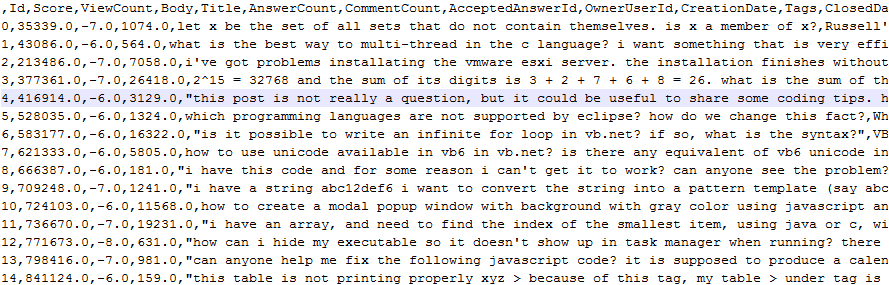
\includegraphics[width=0.8\textwidth]{tag_features_raw}
	\caption{Question without external tags detected.}
	\label{fig:tag_features_raw}
\end{figure}
\begin{figure}[ht]
	\centering
	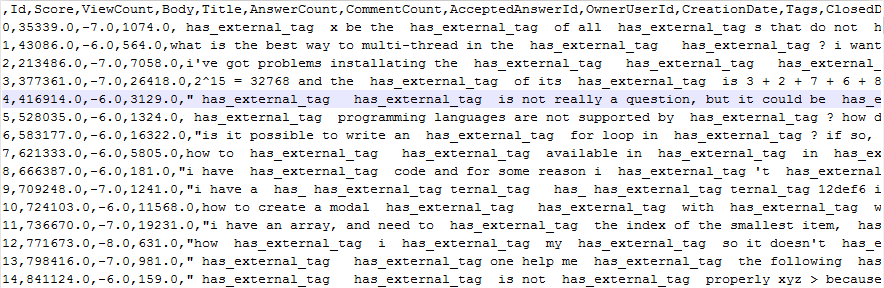
\includegraphics[width=0.8\textwidth]{tag_features_external}
	\caption{Question with external tags detected.}
	\label{fig:tag_features_external}
\end{figure}

\clearpage
\section{Scikit-learns roadmap - Choosing the right estimator}
\label{app:ml_map}
% image of the cheat-sheet from scikit-learn
\begin{figure}[ht]
	\centering
	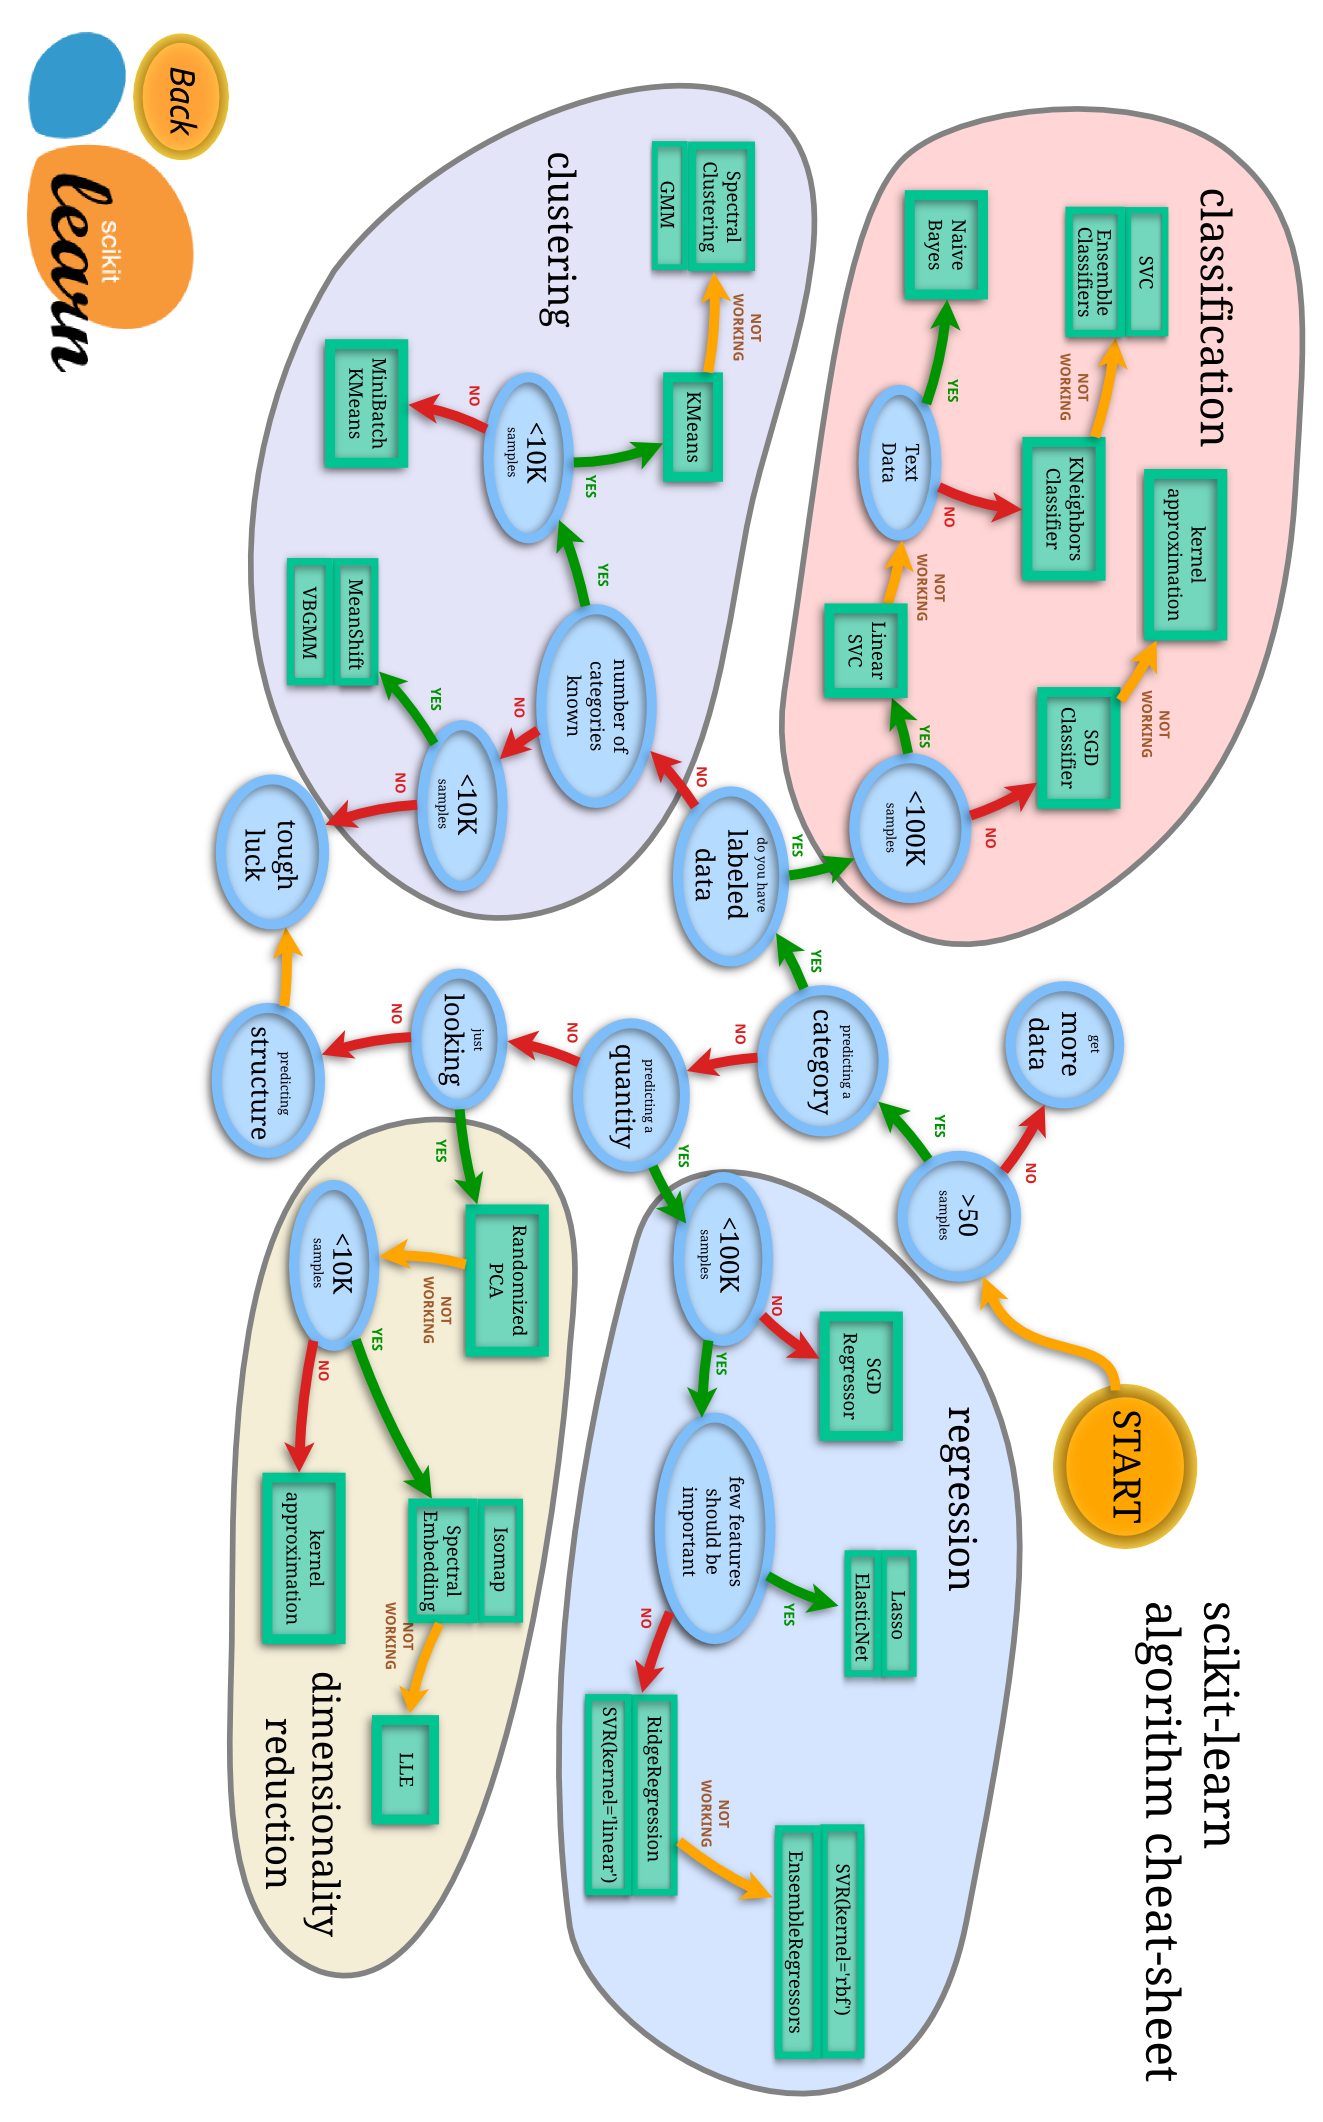
\includegraphics[width=0.645\textwidth]{ml_map}
	\caption[Choosing the right estimator]{Choosing the right estimator \cite{Scikitlearn.org2016i}.}
	\label{fig:ml_map}
\end{figure}

\clearpage
\section{Quick installation guide for Windows x64}
\label{app:installation_windows}
Since Python is much more adapted to *nix systems then Windows, I decided to write a short guide on how to install Python 3.5 and Scikit-learn on Windows. 
This guide is provided as-is, and I make no guarantees that this will result in a functioning installation, but it should at least reduce the problems. 
A presumption here is that the operative system is Windows x64 (if you have x86, you can ignore all the x64 settings).
Before installing anything, download the following:
\begin{itemize}
	\item Python: \url{https://www.python.org/downloads/windows/}. \\
	Select the Python version with "Windows x86-64" in its name.
	\item CygWin: \url{https://cygwin.com/}
	\item MinGW: \url{http://www.mingw.org/}
	\item MySQL connector for Python (Git; only needed for running this project): \\
	\url{https://github.com/mysql/mysql-connector-python}.
	\item x64 version of Numpy and Scipy \cite{Codementor.io2015,Gehrcke2015}: \\ 
	\url{http://www.lfd.uci.edu/~gohlke/pythonlibs/}. \\ 
	The latest available versions at the time of writing is "\emph{numpy-1.11.1rc1+mkl-cp35-cp35m-win\_amd64.whl}" and "\emph{scipy-0.17.1-cp35-cp35m-win\_amd64.whl}".
	\item Scikit-learn (Git): \url{https://github.com/scikit-learn/scikit-learn}
	\item If you do not have a version of Microsoft Visual Studio installed, you need to install Visual Studio 2013 or newer (because compiler requires it)\footnote{
		"vcvarsall.bat needed for python to compile missing from visual studio 2015": \\
		\url{http://stackoverflow.com/q/33323172}
	}.
\end{itemize}
% editor space
\begin{enumerate}
	\item Install Python, update pip, and install these packages: \\
	\emph{pip install -U bs4 pandas nltk matplotlib cython nose nosetests}
	\item Install MinGW.
	 Thereafter select "mingw32-base" under "MinGW Base System".
	In addition, under "MinGW Base System", select all belonging to Class "bin" and "dll"
	\item Install CygWin. 
	During installation, you will be asked what you want to install. 
	Select all entries that contains "gcc", "mingw64", "make", "automake", "lapack" and "openblas".
	The GCC-compilers are used in combination with MinGW, because Scikit-learn needs Fortran, Lapack and OpenBlas for \emph{make} to succeed.
	\item Change to folder with the x64 version of Numpy and Scipy, and install them~\cite{Codementor.io2015,Gehrcke2015}: \\
	\emph{pip install "numpy-1.11.1rc1+mkl-cp35-cp35m-win\_amd64.whl"} \\
	Verify installation: 1. \emph{python}, 2. \emph{import numpy}, 3. \emph{numpy.\_\_version\_\_}. \\
	\emph{pip install "scipy-0.17.1-cp35-cp35m-win\_amd64.whl"} and verify using the same steps, swapping numpy with scipy.
	\item Start CygWin (run as administrator), change to directory containing Scikit-learn and run the following commands: \\
	\emph{python setup.py build}  and \emph{python setup.py install}.
	\item If you want to use \gls{nltk}, you need to run \emph{python}, \emph{import nltk} and \emph{ntlk.download()} to download the corpus.
\end{enumerate}


% backup of various created tables
\begin{comment}

td-10000-Unprocessed
--------------------
Confusion matrix for test set classification:
[[1591  403]
[ 401 1605]]
Accuracy score for test set:
0.799
Classification Report:
			Precision	Recall		F1-score	Support

-1       0.80      0.80      0.80      1994
1       0.80      0.80      0.80      2006

avg / total       0.80      0.80      0.80      4000


Creating singular feature detector:  Code blocks
-----------------------------------------------
Confusion matrix for test set classification:
[[1574  420]
[ 413 1593]]
Accuracy score for test set:
0.79175
Classification Report:
			Precision	Recall		F1-score	Support

-1       0.79      0.79      0.79      1994
1       0.79      0.79      0.79      2006

avg / total       0.79      0.79      0.79      4000


Creating singular feature detector:  Links
-------------------------------------------
Confusion matrix for test set classification:
[[1584  410]
[ 416 1590]]
Accuracy score for test set:
0.7935
Classification Report:
			Precision	Recall		F1-score	Support

-1       0.79      0.79      0.79      1994
1       0.80      0.79      0.79      2006

avg / total       0.79      0.79      0.79      4000


Creating singular feature detector:  Homework
----------------------------------------
Confusion matrix for test set classification:
[[1590  404]
[ 400 1606]]
Accuracy score for test set:
0.799
Classification Report:
			Precision	Recall		F1-score	Support

-1       0.80      0.80      0.80      1994
1       0.80      0.80      0.80      2006

avg / total       0.80      0.80      0.80      4000


Creating singular feature detector:  Numerical
----------------------------------------
Confusion matrix for test set classification:
[[1591  403]
[ 375 1631]]
Accuracy score for test set:
0.8055
Classification Report:
			Precision	Recall		F1-score	Support

-1       0.81      0.80      0.80      1994
1       0.80      0.81      0.81      2006

avg / total       0.81      0.81      0.81      4000


Creating singular feature detector:  Hexadecimal
----------------------------------------
Confusion matrix for test set classification:
[[1591  403]
[ 401 1605]]
Accuracy score for test set:
0.799
Classification Report:
			Precision	Recall		F1-score	Support

-1       0.80      0.80      0.80      1994
1       0.80      0.80      0.80      2006

avg / total       0.80      0.80      0.80      4000


Creating singular feature detector:  Tags
----------------------------------------
Confusion matrix for test set classification:
[[1508  486]
[ 467 1539]]
Accuracy score for test set:
0.76175
Classification Report:
			Precision	Recall		F1-score	Support

-1       0.76      0.76      0.76      1994
1       0.76      0.77      0.76      2006

avg / total       0.76      0.76      0.76      4000


All features using 10k-unprocessed settings
----------------------------------------
Confusion matrix for test set classification:
[[1558  436]
[ 401 1605]]
Accuracy score for test set:
0.79075
Classification Report:
			Precision	Recall		F1-score	Support

-1       0.80      0.78      0.79      1994
1       0.79      0.80      0.79      2006

avg / total       0.79      0.79      0.79      4000


Creating model without stemming, using exhaustive search
------------------------------------------------------------
Confusion matrix for test set classification:
[[1567  427]
[ 408 1598]]
Accuracy score for test set:
0.79125
Classification Report:
			Precision	Recall		F1-score	Support

-1       0.79      0.79      0.79      1994
1       0.79      0.80      0.79      2006

avg / total       0.79      0.79      0.79      4000


td-10k
----------------------------------------
Confusion matrix for test set classification:
[[1558  436]
[ 525 1481]]
Accuracy score for test set:
0.75975
Classification Report:
			Precision	Recall		F1-score	Support

-1       0.75      0.78      0.76      1994
1       0.77      0.74      0.76      2006

avg / total       0.76      0.76      0.76      4000


td-10k-no-stemming
---------------------------------------------
Confusion matrix for test set classification:
[[1568  426]
[ 408 1598]]
Accuracy score for test set:
0.7915
Classification Report:
			Precision	Recall		F1-score	Support

-1       0.79      0.79      0.79      1994
1       0.79      0.80      0.79      2006

avg / total       0.79      0.79      0.79      4000


10k-sgd-loss-log
----------------------------------------
Confusion matrix for test set classification:
[[1610  384]
[ 594 1412]]
Accuracy score for test set:
0.7555
Classification Report:
			Precision	Recall		F1-score	Support

-1       0.73      0.81      0.77      1994
1       0.79      0.70      0.74      2006

avg / total       0.76      0.76      0.75      4000


10k-unprocessed-sgd
------------------
Confusion matrix for test set classification:
[[1607  387]
[ 418 1588]]
Accuracy score for test set:
0.79875
Classification Report:
			Precision	Recall		F1-score	Support

-1       0.79      0.81      0.80      1994
1       0.80      0.79      0.80      2006

avg / total       0.80      0.80      0.80      4000


10k-unprocessed-sgd-log-loss
------------------
Confusion matrix for test set classification:
[[1607  387]
[ 418 1588]]
Accuracy score for test set:
0.79875
Classification Report:
			Precision	Recall		F1-score	Support

-1       0.79      0.81      0.80      1994
1       0.80      0.79      0.80      2006

avg / total       0.80      0.80      0.80      4000


td-10k-all-features-occurrence-only
------------------
Confusion matrix for test set classification:
[[1268  403]
[ 329 1512]]
Accuracy score for test set:
0.791571753986
Classification Report:
			Precision	Recall		F1-score	Support

-1.0       0.79      0.76      0.78      1671
1.0       0.79      0.82      0.81      1841

avg / total       0.79      0.79      0.79      3512


td-10l-unprocessed-codeblocks
------------------------------------
Confusion matrix for test set classification:
[[793 195]
[218 765]]
Accuracy score for test set:
0.790461694571
Classification Report:
			Precision	Recall		F1-score	Support

-1.0       0.78      0.80      0.79       988
1.0       0.80      0.78      0.79       983

avg / total       0.79      0.79      0.79      1971


td-10l-unprocessed-hexadecimal
------------------------------------
Confusion matrix for test set classification:
[[21  0]
[ 6  5]]
Accuracy score for test set:
0.8125
Classification Report:
			Precision	Recall		F1-score	Support

-1.0       0.78      1.00      0.88        21
1.0       1.00      0.45      0.62        11

avg / total       0.85      0.81      0.79        32


td-10l-unprocessed-homework
------------------------------------
Confusion matrix for test set classification:
[[50  6]
[ 7 12]]
Accuracy score for test set:
0.826666666667
Classification Report:
			Precision	Recall		F1-score	Support

-1.0       0.88      0.89      0.88        56
1.0       0.67      0.63      0.65        19

avg / total       0.82      0.83      0.83        75


td-10l-unprocessed-links
------------------------------------
Confusion matrix for test set classification:
[[ 87  64]
[ 30 335]]
Accuracy score for test set:
0.817829457364
Classification Report:
			Precision	Recall		F1-score	Support

-1.0       0.74      0.58      0.65       151
1.0       0.84      0.92      0.88       365

avg / total       0.81      0.82      0.81       516


td-10l-unprocessed-numeric
------------------------------------
Confusion matrix for test set classification:
[[1043  111]
[ 256  395]]
Accuracy score for test set:
0.796675900277
Classification Report:
			Precision	Recall		F1-score	Support

-1.0       0.80      0.90      0.85      1154
1.0       0.78      0.61      0.68       651

avg / total       0.79      0.80      0.79      1805


td-10l-unprocessed-tags
------------------------------------
Confusion matrix for test set classification:
[[1487  498]
[ 442 1567]]
Accuracy score for test set:
0.764646970456
Classification Report:
			Precision	Recall		F1-score	Support

-1.0       0.77      0.75      0.76      1985
1.0       0.76      0.78      0.77      2009

avg / total       0.76      0.76      0.76      3994

td-10l-unprocessed-all-features
------------------------------------
Confusion matrix for test set classification:
[[1284  387]
[ 342 1499]]
Accuracy score for test set:
0.792425968109
Classification Report:
			Precision	Recall		F1-score	Support

-1.0       0.79      0.77      0.78      1671
1.0       0.79      0.81      0.80      1841

avg / total       0.79      0.79      0.79      3512


td-10l-unprocessed-up-codeblocks
------------------------------------
Confusion matrix for test set classification:
[[786 202]
[215 768]]
Accuracy score for test set:
0.788432267884
Classification Report:
			Precision	Recall		F1-score	Support

-1.0       0.79      0.80      0.79       988
1.0       0.79      0.78      0.79       983

avg / total       0.79      0.79      0.79      1971


td-10l-unprocessed-up-hex
------------------------------------
Confusion matrix for test set classification:
[[21  0]
[ 6  5]]
Accuracy score for test set:
0.8125
Classification Report:
			Precision	Recall		F1-score	Support

-1.0       0.78      1.00      0.88        21
1.0       1.00      0.45      0.62        11

avg / total       0.85      0.81      0.79        32


td-10l-unprocessed-up-homework
------------------------------------
Confusion matrix for test set classification:
[[52  4]
[ 8 11]]
Accuracy score for test set:
0.84
Classification Report:
					precision    	recall  	f1-score   	support

-1.0       			0.87      		0.93      	0.90        56
1.0       			0.73      		0.58      	0.65        19

avg / total       	0.83     	 	0.84      	0.83        75


td-10l-unprocessed-up-links
------------------------------------
Confusion matrix for test set classification:
[[ 95  56]
[ 28 337]]
Accuracy score for test set:
0.837209302326
Classification Report:
			Precision	Recall		F1-score	Support

-1.0       0.77      0.63      0.69       151
1.0       0.86      0.92      0.89       365

avg / total       0.83      0.84      0.83       516


td-10l-unprocessed-up-numeric
------------------------------------
Confusion matrix for test set classification:
[[1044  110]
[ 247  404]]
Accuracy score for test set:
0.802216066482
Classification Report:
			Precision	Recall		F1-score	Support

-1.0       0.81      0.90      0.85      1154
1.0       0.79      0.62      0.69       651

avg / total       0.80      0.80      0.80      1805


td-10l-unprocessed-up-tags
------------------------------------
Confusion matrix for test set classification:
[[1559  426]
[ 398 1611]]
Accuracy score for test set:
0.793690535804
Classification Report:
			Precision	Recall		F1-score	Support

-1.0       0.80      0.79      0.79      1985
1.0       0.79      0.80      0.80      2009

avg / total       0.79      0.79      0.79      3994

\end{comment}


\begin{comment}
\begin{table}[!htb]
\caption{Confusion Matrix for xxxxx.}
\begin{minipage}{.5\linewidth}
\caption{Unprocessed dataset}
\centering
\begin{tabular}{| c | c | c |}
\hline
Actual 		& Predicted: -1	& Predicted: 1	\\ \hline
-1			& xx			& xx			\\ \hline
1			& xx			& xx			\\ \hline
\end{tabular}
\end{minipage}%
\begin{minipage}{.5\linewidth}
\centering
\caption{All features}
\begin{tabular}{| c | c | c |}
\hline
Actual 		& Predicted: -1	& Predicted: 1	\\ \hline
-1			& xx			& xx			\\ \hline
1			& xx			& xx			\\ \hline
\end{tabular}
\end{minipage} 
\end{table}	

Amount of features before anything was done to the text: 69766 - CountVectorizer(analyzer='word') - \%
Amount of features after adding stop word (English): 69462 - CountVectorizer(analyzer='word', stop\_words="english") - \%
Amount of features after removing code block, hexadecimals and numeric values: 27624 - \%
Amount of features after setting minimum document frequency: 440 - CountVectorizer(analyzer='word', min\_df=0.01, stop_words='english') - \%


Originally tagged questions as good/bad, but then switched to +/-1 due to considering switching to LibSVM.
\end{comment}
